\documentclass[english,xcolor=dvipsnames]{beamer}
% load package with ``framed'' and ``numbered'' option.
\usepackage[numbered,framed,autolinebreaks,useliterate]{mcode}
\usepackage[orientation=landscape,size=custom,width=16,height=9,scale=0.48,debug]{beamerposter}
\usepackage[T1]{fontenc}
\usepackage[latin9]{inputenc}
\usepackage{amsthm}
\usepackage{amsmath}
\usepackage{amssymb}
\usepackage{bookmark}
\usepackage{graphics,graphicx}
\usepackage{pstricks,pst-node,pst-tree}
\usefonttheme{serif}
\usepackage{palatino}
\usepackage{tikz}
\usetikzlibrary{shapes,arrows}
\usetikzlibrary{positioning}
%\usepackage[margin=.5cm]{geometry}

\definecolor{dgreen}{rgb}{0.,0.6,0.}
\definecolor{forest}{RGB}{34.,139.,34.}
\definecolor{byublue}{RGB}{0.,30.,76.}
\definecolor{dukeblue}{RGB}{0.,0.,156.}
%\usetheme{Ilmenau}
\usetheme{Warsaw}
\usecolortheme[named=dukeblue]{structure}
%\usecolortheme[named=RawSienna]{structure}
%\usecolortheme[named=byublue]{structure}
\setbeamertemplate{navigation symbols}{}
\setbeamertemplate{footline}{}
\setbeamercovered{transparent}

%%%%%%%%%%%%%%%%%%%%%%%%%%%%%%%%%%%%%%%%%%%%%%%%
% NOTE: With Ilmenau style, to get the bullets %
% looking right, do one section and one sub-   %
% section for each set of bullets              %
%%%%%%%%%%%%%%%%%%%%%%%%%%%%%%%%%%%%%%%%%%%%%%%%

\begin{document}
\begin{frame}
\title{Introduction to Function Optimization}
\author{
	Tyler Ransom\\
	\emph{Duke University}\\
%    \today \\
%    \vspace{10cm}
}
\titlepage
\end{frame}

\begin{frame}{Outline}
\begin{itemize}
	\item Functional Optimization Basics
	\item Optimizing Functions in Matlab
	\item Compare/Contrast \texttt{fminsearch}, \texttt{fminunc}, and \texttt{fmincon}
	\item Discuss \texttt{fsolve}
	\item Determining if your optimizer has given a good solution
	\item Debugging Programs in Matlab
\end{itemize}
\end{frame}

\begin{frame}{Basics of functional optimization}
	\begin{itemize}
		\item All econometric estimators are either minima of some error function or maxima of some likelihood function
		\item Some estimators (e.g. OLS, GMM) have \textbf{closed form} solutions for the extremum value
		\item Other estimators (e.g. MLE, some NLLS) require \textbf{numerical methods} to find the extremum value
		\item Matlab has a number of different algorithms to numerically find extrema
	\end{itemize}
\end{frame}

\begin{frame}{Graphical depiction of the optimization problem}
\centering
\includegraphics[width=0.70\textwidth]{LogLVOacac.jpg}\\
\scriptsize{Source: \texttt{http://earlelab.rit.albany.edu/images.html}}
\end{frame}

\begin{frame}{How numerical optimization works}
	\begin{itemize}
		\item User provides an objective function and a starting value
		\item The optimizer then calculates the magnitude and direction of the gradient vector at the starting value
		\item Given these values of the gradient vector, it decides 
		\begin{enumerate}
			\item in which direction to move to get closer to the optimum
			\item how far it should move to get closer to the optimum
		\end{enumerate}
		\item Given the magnitude and direction of the gradient vector at the new point, it repeats these steps until convergence is achieved 
	\end{itemize}
\end{frame}

\begin{frame}{Determining convergence}
There are generally three ways to determine if a numerical optimization algorithm has reached the optimum
	\begin{enumerate}
		\item The gradient vector (or Jacobian matrix) is numerically close zero
		\begin{itemize}
			\item Intuition: $f^\prime (x) = 0 \, \Rightarrow \, x$ may be an extremum
		\end{itemize}
		\item The location of the previous guess is numerically close to the location of the updated guess
		\begin{itemize}
			\item Intuition: The optimizer didn't move very far in updating the guess, so we're probably close to the answer
		\end{itemize}
		\item The value of the objective function at the previous guess is numerically close to the value of the objective function at the updated guess
		\begin{itemize}
			\item Intuition: The objective function is flat in the area of the previous and updated guesses, which is kind of like having a gradient of zero
		\end{itemize} 
	\end{enumerate}
Note that ``numerically close'' generally refers to being within $10^{-6}$\\
\end{frame}

\begin{frame}{Is the extremum global?}
\begin{itemize}
	\item Note that in the previous slide, no mention of second-order conditions was ever made
	\item Hence, it is unclear if the answer our optimizer gave is a local optimum, a saddle point, or a global optimum
	\item Luckily, most common econometric estimators have been proven to have globally concave objective functions
	\item If you are unsure whether or not your objective function is globally concave, you can try different sets of starting values and see how much the answers differ
\end{itemize}
\end{frame}

\begin{frame}[fragile]{Optimization functions in Matlab}
\begin{itemize}
	\item All of Matlab's optimizers find \emph{minima}. If a user wants to find the maximum, she must minimize the \emph{negative} of her objective function
	\item The three most common optimizers are
\end{itemize}
\begin{lstlisting}
fminsearch %Find minimum of unconstrained multivariable function using derivative-free method
fminunc    %Find minimum of unconstrained nonlinear multivariable function
fmincon    %Find minimum of constrained nonlinear multivariable function
\end{lstlisting}
\mcode{fminunc} is by far the most popular optimization algorithm in Matlab, but we'll discuss the pros and cons to each
\end{frame}

\begin{frame}[fragile]{How to call an optimizer in Matlab}
The syntax for calling an optimizer to estimate a general function is
\begin{lstlisting}
[x,fval,exitflag,output] = fminwhatever('fun',x0,options,varargin)
\end{lstlisting}
where \\
\mcode{x} is the vector of parameter estimates\\
\mcode{fval} is the value of the objective function at the parameter estimates\\
\mcode{exitflag} is an integer displaying the reason optimization stopped\\
\mcode{output} is a structure containing information about the optimization\\
\mcode{fun} is a function m-file (or function handle) that has the objective function as an output and the parameter vector as an input\\
\mcode{x0} is the starting value for the optimization routine\\
\mcode{options} is a structure of estimation options\\
\mcode{varargin} is whatever other inputs go in to \mcode{fun} (e.g. data matrices, rhs variables, other non-estimated parameters)\\
\end{frame}

\begin{frame}[fragile]{Example: \texttt{fminsearch}}
Let's look at how to estimate OLS on the model $Y=X\beta+\varepsilon$ using \mcode{fminsearch}, where $\beta$ is two-dimensional
\begin{itemize}
	\item In the script m-file, 
\end{itemize}
\begin{lstlisting}
[beta,SSE] = fminsearch('OLS1',.5*ones(2,1),[],X,Y);
\end{lstlisting}
The function m-file then looks like
\begin{lstlisting}
function SSE = OLS1(beta,X,Y)
SSE = (Y-X*beta)'*(Y-X*beta);
\end{lstlisting}
\end{frame}

\begin{frame}[fragile]{\texttt{fminsearch} optimization options}
\begin{lstlisting}
Display     %allows user to display iterations 
FunValCheck %Check whether objective function values are valid
MaxFunEvals %Maximum number of function evaluations allowed (default is 200*numberOfVariables)
MaxIter     %Maximum number of iterations allowed (default value is 200*numberOfVariables)
TolFun      %Termination tolerance on the function value (default is 1e-4)
TolX        %Termination tolerance on x (default value is 1e-4)
\end{lstlisting}
Example of how to implement optimization options (\mcode{optimset} command):
\begin{lstlisting}
o1 = optimset('Display','iter','MaxFunEvals',1e6,'TolFun',1e-6);
[beta,SSE] = fminsearch('OLS1',.5*ones(2,1),o1,X,Y);
\end{lstlisting}
\end{frame}

\begin{frame}[fragile]{\texttt{fminunc}}
\begin{itemize}
	\item Portmanteau of ``Functional MINimization UNConstrained''
	\item \mcode{fminunc} is the best optimizer for well-behaved functions
	\item It has two different optimization algorithms: ``medium scale'' and ``large scale''
	\item \textbf{medium scale}: Solver approximates the gradient and hessian, and uses a quasi-Newton method for searching
	\item \textbf{large scale}: User supplies the analytical gradient and/or hessian, and the solver uses a trust-region algorithm
	\item The medium scale algorithm is generally OK to use for basic econometric estimators. However, optimization moves much more quickly in the large scale algorithm, so if your objective function is easy enough, you should supply the gradient.
\end{itemize}
\end{frame}

\begin{frame}[fragile]{\texttt{fminunc} optimization options}
In addition to the options for \mcode{fminsearch}, \mcode{fminunc} has specific options:
\begin{lstlisting}
DerivativeCheck	%Compare user-supplied gradient to numerical gradient
GradObj         %Use the user-supplied gradient
LargeScale      %Use large-scale algorithm
\end{lstlisting}
\begin{itemize}
	\item There are many more options, but the ones listed above are the main ones to use
	\item Use \mcode{optimset} to initialize the options in the same way as the \mcode{fminsearch} example
	\item Additionally, \mcode{fminunc} has two more outputs than \mcode{fminsearch}:
\end{itemize}
\begin{lstlisting}
[x,fval,exitflag,output,gradient,hessian] = fminunc('fun',x0,options,varargin)
\end{lstlisting}
The hessian is particularly useful for statistical inference (i.e. std. errors)
\end{frame}

\begin{frame}[fragile]{\texttt{fminsearch} vs. \texttt{fminunc}}
\begin{columns}
\column{3in}
\mcode{fminsearch}
\begin{itemize}
	\item Simplex search algorithm is more robust than \mcode{fminunc}, particularly in the presence of functional abnormalities
	\item Particularly useful for finding reasonable starting values for \mcode{fminunc}
	\item Runs extremely slowly and inefficiently as the dimension of parameters increases
	\item Doesn't estimate a hessian, so can't get standard errors on parameter estimates
\end{itemize}
\column{3in}
\mcode{fminunc}
\begin{itemize}
	\item Uses a line search or trust region algorithm (similar to the 2nd slide of today's lecture) that works very well for well-behaved functions (like those in traditional econometrics)
	\item Objective function must be continuous
	\item Starting values need to be reasonable or solution may not be correct
	\item Can handle any number of parameters
	\item Estimates a numerical hessian which can be used for inference
\end{itemize}
\end{columns}
\end{frame}

\begin{frame}[fragile]{\texttt{fmincon} optimization problem}
\begin{itemize}
	\item Portmanteau of ``Functional MINimization CONstrained''
	\item \mcode{fmincon} performs optimization of the following form:
\end{itemize}
\begin{equation*}
\min_{x} f(x) \, \textrm{subject to Constraints}
\end{equation*}
where Constraints is any one or more of
\begin{itemize}
	\item $c(x)\leq0$, \quad $c(x)$ is an output of a function m-file which forms the nonlinear constraint function
	\item $ceq(x)=0$, \quad $ceq(x)$ is another output of the $c(x)$ function m-file
	\item $A\cdot x\leq b$, \quad $A$ and $b$ are a matrix and vector, respectively
	\item $Aeq\cdot x= beq$, \quad $Aeq$ and $beq$ are a matrix and vector, respectively
	\item $lb\leq x \leq ub$, \quad $lb$ and $ub$ are each vectors the same size as $x$
\end{itemize}
\end{frame}

\begin{frame}[fragile]{\texttt{fmincon} syntax}
\begin{lstlisting}
[x,fval,exitflag,output,lambda,gradient,hessian] = fmincon('fun',x0,A,b,Aeq,beq,lb,ub,'nonlcon',options,varargin of 'fun');
\end{lstlisting}
\begin{itemize}
	\item Outputs are same as \mcode{fminunc}, with an additional \texttt{lambda} which is the Lagrange multipliers from the constraint function
	\item Note that the ordering of the inputs is quite different from \mcode{fminunc}, namely that all of the constraints come after the starting values and before the optimization options (and other inputs to \mcode{'fun'})
	\item The constraint matrices \mcode{A,b,Aeq,beq,lb,ub} line up with the constraints from the previous slide---but at least one is required
	\begin{itemize}
		\item Put an empty matrix (\mcode{[]}) for any of the \mcode{A,b,Aeq,beq,lb,ub,'nonlcon'} you're not using
	\end{itemize}
	\item \mcode{'nonlcon'} refers to $c(x)\leq0$ or $ceq(x)=0$ from the previous slide, where $c$ and $ceq$ are outputs of \mcode{nonlcon}
\end{itemize}
\end{frame}

\begin{frame}[fragile]{\texttt{fmincon} optimization options}
\begin{itemize}
	\item \texttt{fmincon} has four different optimization algorithms (instead of large and medium scale in \texttt{fminunc})
	\item Like \texttt{fminunc}, user can provide gradient and hessian to \texttt{fmincon}
	\item The gradient and hessian are the derivatives of the \emph{Lagrangian}, not just the objective function
	\item As with \texttt{fminunc}, the more information provided by the user, the faster/better the optimizer solves
	\item \texttt{fmincon}-specific optimization options:
\end{itemize}
\begin{lstlisting}
GradConstr  %gradient of constraint function; similar to GradObj
TolCon      %tolerance on constraint violation (similar to TolX, TolFun)
UseParallel %estimate numerical gradients via parallel computing
\end{lstlisting}
There are other options specific to each algorithm which we won't go through
\end{frame}

\begin{frame}[fragile]{\texttt{fmincon} in perspective}
\begin{itemize}
	\item \texttt{fmincon} requires at least one type of constraint
	\item Constrained optimization typically takes longer than unconstrained optimization
	\item Sometimes it is possible to re-parameterize a constrained problem into becoming an unconstrained one
	\item Doing so may save computational time, though this savings varies from problem to problem
	\item You will probably never use \texttt{fmincon} (outside of this class) because most standard econometric problems are simple enough for \texttt{fminunc} to handle
	\item At the end of the day, remember that optimization can be more of an art than a science
\end{itemize}
\end{frame}

\begin{frame}[fragile]{\texttt{fsolve}}
\begin{itemize}
	\item Portmanteau of ``Function SOLVEr''
	\item \mcode{fsolve} is an optimizer for nonlinear systems of equations
	\item It solves for the vector $x$ such that $f\left(x\right)=0$
	\item Unlike the other functional optimizers we've gone over, \mcode{fsolve} requires both inputs and outputs to be vector-valued
	\item It has three different optimization algorithms: ``trust-region-dogleg'' (default), ``trust-region-reflective'', and ``levenberg-marquardt''
\end{itemize}
\end{frame}

\begin{frame}[fragile]{\texttt{fsolve} optimization options}
\mcode{fsolve} has similar options to the other functional optimizers in Matlab:
\begin{lstlisting}
DerivativeCheck	%Compare user-supplied first derivatives to numerical first derivatives
Jacobian        %Use the user-supplied Jacobian (matrix of first derivatives)
\end{lstlisting}
\begin{itemize}
	\item There are many more options, but the ones listed above are the main ones to use
	\item Use \mcode{optimset} to initialize the options in the same way as the other examples
	\item \mcode{fsolve} has one more output than \mcode{fminsearch}:
\end{itemize}
\begin{lstlisting}
[x,fval,exitflag,output,jacobian] = fsolve('fun',x0,options,varargin)
\end{lstlisting}
The Jacobian can be useful for certain applications
\end{frame}

\begin{frame}{MLE using \texttt{fsolve}}
\begin{itemize}
	\item Recall that MLE is just a solution to a system of nonlinear equations (which may not have a closed-form solution)
	\item We could use \texttt{fsolve} to find the solution, where $F\left(x\right)$ is the system of first-derivatives
	\item However, we need the solution to be a maximum, so we would need the \texttt{fsolve} Jacobian (the Hessian of the likelihood) to be negative definite
	\item I can't figure out how to impose this restriction in \texttt{fsolve}
	\item Hence, it's not a good idea in general to use \texttt{fsolve} for MLE
	\item In practice, \texttt{fsolve} is commonly used in IO to find FOCs in profit maximization problems, where the FOCs may not have a closed-form solution
\end{itemize}
\end{frame}

\begin{frame}{Exit Flags}
The following table summarizes the exit flags that can be recovered through the third output of a minimizer
\begin{center}
\begin{tabular}{|c|c|}
\hline 
Exit flag & Description\\
\hline 
-4 & Line search can't find a suitable direction\\
\hline 
-3 & Objective function went below -$10^{20}$\\
\hline 
-2 & No feasible point was found\\
\hline 
-1 & Algorithm was terminated by the output function\\
\hline 
0 & iterations $>$ MaxIter or funEvals $>$ MaxFunEvals\\
\hline 
1 & solution found (gradient$<$ TolFun tolerance)\\
\hline 
2 & Change in $x$ was smaller than the TolX tolerance\\
\hline 
3 & Change in the Fun value $<$ TolFun tolerance\\
\hline 
4 & Magnitude of search direction $<$ specified tolerance.\\
\hline 
5 & Predicted decrease in Fun$<$ TolFun tolerance\\
\hline 
\end{tabular}
\end{center}
\end{frame}

\begin{frame}{Optimization output}
The following table summarizes the output that can be recovered through the fourth output of a minimizer
\begin{center}
\begin{small}
\begin{tabular}{|c|c|}
\hline 
Output & Description\\
\hline 
\hline 
iterations & Number of iterations taken\\
\hline 
funcCount & Number of function evaluations\\
\hline 
firstorderopt & Measure of first-order optimality\\
\hline 
algorithm & Optimization algorithm used\\
\hline 
cgiterations & Total number of PCG iterations (large-scale algorithm only)\\
\hline 
stepsize & Final displacement in x (only for certain algorithms)\\
\hline 
lssteplength & Size of line search step relative to search direction (active-set
algorithm only)\\
\hline 
constrviolation & Maximum of constraint functions\\
\hline 
message & Exit message\\
\hline 
\end{tabular}
\end{small}
\end{center}
\end{frame}

\begin{frame}[fragile]{Choosing optimization options in a GUI environment}
\begin{itemize}
	\item Matlab has a user-friendly optimization tool (type ``\mcode{optimtool}'' in the command window)
	\item Users can graphically see all the options available for each optimizer
	\item Matlab can generate code for the optimization so users don't have to worry about syntax errors
\end{itemize}
\end{frame}


\begin{frame}{Debugging in Matlab}
% Define block styles
\tikzstyle{block} = [rectangle, draw, fill=blue!20, 
    text width=16em, rounded corners, minimum height=4em]
\tikzstyle{line} = [draw, -latex']
\tikzstyle{block2} = [rectangle, draw, fill=red!20, 
    text width=16em, rounded corners, minimum height=4em]
Recall this diagram illustrating how functions are called in Matlab:
\begin{tikzpicture}[node distance = .5cm, auto]
\tikzstyle{every node}=[font=\small]
    % Place nodes
    \node [block] (script) {\textbf{Script m-file (\texttt{example.m})} \\ . \\ . \\ . \\ \texttt{B=my\_function(A)}};
    \node [block2, below right = of script] (function) {\textbf{Function m-file (\texttt{my\_function.m})} \\ \texttt{out1=my\_function(inp1)}\\  \texttt{out1 = (inp1>0);} \\ \texttt{end}};
    \node [block, below left = of function] (script2) {\textbf{Script m-file (continued)} \\ \texttt{B=my\_function(A)} \\ . \\ . \\ . };

    % Draw edges
    \path [line] (script) -- (function);
    \path [line] (function) -- (script2);
\end{tikzpicture}
\end{frame}

\begin{frame}[fragile]{Debugging in Matlab}
\begin{itemize}
	\item Suppose a user wants to try to fix a problem nested deep in a function called by an optimizer
	\item Recall from the previous slide that the workspace inside a function only includes the inputs passed to the function (and/or global variables)
	\item Hence, a user needs to get inside the function to identify any problems occurring within the function
	\item The only problem is telling Matlab to stop at the right spot (inside the function)
	\item Matlab has a very useful debugging system for accomplishing this task
\end{itemize}
\end{frame}

\begin{frame}[fragile]{Debugging in Interactive Mode}
\centering
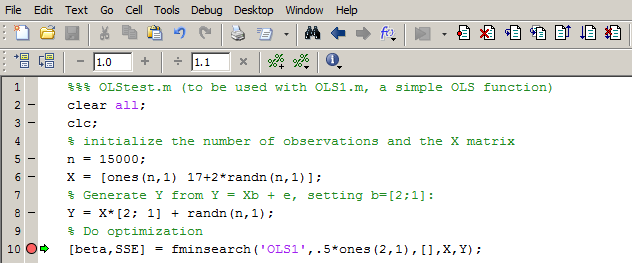
\includegraphics[width=0.70\textwidth]{dbscreen1.png}\\
\begin{enumerate}
	\item Begin by placing a breakpoint on the line where the optimization is being called, and press the play button
\end{enumerate}
\end{frame}

\begin{frame}[fragile]{Debugging in Interactive Mode}
\centering
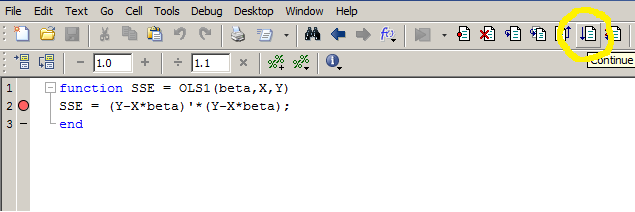
\includegraphics[width=0.70\textwidth]{dbscreen2.png}\\
\begin{enumerate}
\setcounter{enumi}{1}
	\item Next, place a breakpoint somewhere in your function m-file, and click ``continue''
\end{enumerate}
\end{frame}

\begin{frame}[fragile]{Debugging in Interactive Mode}
\centering
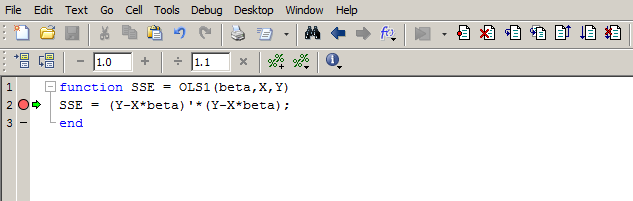
\includegraphics[width=0.70\textwidth]{dbscreen3.png}\\
\begin{enumerate}
\setcounter{enumi}{2}
	\item Matlab has stopped on the first line of the function. The user can now examine the workspace to identify inconsistencies
	\item To quit debug mode, click on the far right icon (to the right of ``continue'')
	\item To clear breakpoints, click on the other icon with the red x
\end{enumerate}
\end{frame}

\begin{frame}[fragile]{Debugging commands}
\begin{itemize}
	\item Debugging is much easier to do in interactive mode, but can also be done from the command line (i.e. in batch mode) using the following commands:
\end{itemize}
\begin{lstlisting}
dbstop in [file] at [line number] %sets a debug break point at the specified location
dbcont   %continues execution from the previous breakpoint until the next
dbquit   %quits debug mode
dbclear  %clear breakpoints in certain (or all) files
keyboard %quick-and-dirty way of debugging; hands control over to the keyboard
\end{lstlisting}
\end{frame}

\begin{frame}[fragile]{Debugging commands}
\begin{itemize}
	\item The sequence of debugging shown in interactive mode can be accomplished equally from the command line through this sequence of debug commands:
\end{itemize}
\begin{lstlisting}
dbstop in OLStest at 10 %set first breakpoint
OLStest                 %execute the script
dbstop in OLS1 at 2     %set second breakpoint
dbcont                  %continue
dbquit                  %exit debug mode
dbclear all             %clear all breakpoints
\end{lstlisting}
\end{frame}


\end{document}
